\documentclass{article}[18pt]
\ProvidesPackage{format}
%Page setup
\usepackage[utf8]{inputenc}
\usepackage[margin=0.7in]{geometry}
\usepackage{parselines} 
\usepackage[english]{babel}
\usepackage{fancyhdr}
\usepackage{titlesec}
\hyphenpenalty=10000

\pagestyle{fancy}
\fancyhf{}
\rhead{Sam Robbins}
\rfoot{Page \thepage}

%Characters
\usepackage{amsmath}
\usepackage{amssymb}
\usepackage{gensymb}
\newcommand{\R}{\mathbb{R}}

%Diagrams
\usepackage{pgfplots}
\usepackage{graphicx}
\usepackage{tabularx}
\usepackage{relsize}
\pgfplotsset{width=10cm,compat=1.9}
\usepackage{float}

%Length Setting
\titlespacing\section{0pt}{14pt plus 4pt minus 2pt}{0pt plus 2pt minus 2pt}
\newlength\tindent
\setlength{\tindent}{\parindent}
\setlength{\parindent}{0pt}
\renewcommand{\indent}{\hspace*{\tindent}}

%Programming Font
\usepackage{courier}
\usepackage{listings}
\usepackage{pxfonts}

%Lists
\usepackage{enumerate}
\usepackage{enumitem}

% Networks Macro
\usepackage{tikz}


% Commands for files converted using pandoc
\providecommand{\tightlist}{%
	\setlength{\itemsep}{0pt}\setlength{\parskip}{0pt}}
\usepackage{hyperref}

% Get nice commands for floor and ceil
\usepackage{mathtools}
\DeclarePairedDelimiter{\ceil}{\lceil}{\rceil}
\DeclarePairedDelimiter{\floor}{\lfloor}{\rfloor}

% Allow itemize to go up to 20 levels deep (just change the number if you need more you madman)
\usepackage{enumitem}
\setlistdepth{20}
\renewlist{itemize}{itemize}{20}

% initially, use dots for all levels
\setlist[itemize]{label=$\cdot$}

% customize the first 3 levels
\setlist[itemize,1]{label=\textbullet}
\setlist[itemize,2]{label=--}
\setlist[itemize,3]{label=*}

% Definition and Important Stuff
% Important stuff
\usepackage[framemethod=TikZ]{mdframed}

\newcounter{theo}[section]\setcounter{theo}{0}
\renewcommand{\thetheo}{\arabic{section}.\arabic{theo}}
\newenvironment{important}[1][]{%
	\refstepcounter{theo}%
	\ifstrempty{#1}%
	{\mdfsetup{%
			frametitle={%
				\tikz[baseline=(current bounding box.east),outer sep=0pt]
				\node[anchor=east,rectangle,fill=red!50]
				{\strut Important};}}
	}%
	{\mdfsetup{%
			frametitle={%
				\tikz[baseline=(current bounding box.east),outer sep=0pt]
				\node[anchor=east,rectangle,fill=red!50]
				{\strut Important:~#1};}}%
	}%
	\mdfsetup{innertopmargin=10pt,linecolor=red!50,%
		linewidth=2pt,topline=true,%
		frametitleaboveskip=\dimexpr-\ht\strutbox\relax
	}
	\begin{mdframed}[]\relax%
		\centering
		}{\end{mdframed}}



\newcounter{lem}[section]\setcounter{lem}{0}
\renewcommand{\thelem}{\arabic{section}.\arabic{lem}}
\newenvironment{defin}[1][]{%
	\refstepcounter{lem}%
	\ifstrempty{#1}%
	{\mdfsetup{%
			frametitle={%
				\tikz[baseline=(current bounding box.east),outer sep=0pt]
				\node[anchor=east,rectangle,fill=blue!20]
				{\strut Definition};}}
	}%
	{\mdfsetup{%
			frametitle={%
				\tikz[baseline=(current bounding box.east),outer sep=0pt]
				\node[anchor=east,rectangle,fill=blue!20]
				{\strut Definition:~#1};}}%
	}%
	\mdfsetup{innertopmargin=10pt,linecolor=blue!20,%
		linewidth=2pt,topline=true,%
		frametitleaboveskip=\dimexpr-\ht\strutbox\relax
	}
	\begin{mdframed}[]\relax%
		\centering
		}{\end{mdframed}}
\lhead{Networks and Systems - Compiler Design}


\begin{document}
\begin{center}
\underline{\huge Top Down Analysis}
\end{center}
Top down constriction of a parse tree:
\begin{itemize}
	\item Start with the root, labelled by the starting symbol
	\item Repeatedly perform the following steps:
	\begin{enumerate}
		\item At internal node N, labelled with non-terminal A
		\begin{itemize}
			\item Select one of the production rules for A
			\item Construct children at N for the symbols in the right part of this production rule
		\end{itemize}
		\item Find the next node to construct a subtree
		\begin{itemize}
			\item Typically the leftmost unexpanded non-terminal of the current tree
		\end{itemize}
	\end{enumerate}
\end{itemize}
During the construction of the parse tree the current terminal of the input that is being scanned is called the lookahead symbol\\
\\
Our aim during top-down parsing - to construct the parse tree, such that the string generated by the parse tree matches the input string\\
\\
For a match to occur - the starting symbol stmt must derive a string that starts with for\\
\\
When a node in the parse tree:
\begin{itemize}
	\item Is labelled with a terminal
	\item Matches the lookahead symbol
\end{itemize}
Then
\begin{itemize}
	\item The lookahead becomes the next terminal in the input
	\item We consider the next child in the parse tree
\end{itemize}
When a node in the parse tree is labelled with a non-terminal then:
\begin{itemize}
	\item We repeat by selecting one of its production rules
	\item Special case: $A\rightarrow \epsilon$ - we choose it when nothing else can be used
\end{itemize}
In general:
\begin{itemize}
	\item Many possibilities for a production at a non-terminal
	\item The selection of one of them may involve trial and error
\end{itemize}
A selected production is unsuitable if after using this production, we can't complete the tree to match the whole input string\\
\\
If a selected production is unsuitable, backtrack and try another production until we 
\begin{itemize}
	\item either match the input string
	\item or we report error (input string not in the language)
\end{itemize}
\section{Recursive descent parsing}
\begin{itemize}
	\item A top-down parsing method, using recursive procedures to process the input
	\item One procedure for each non-terminal of the grammar
	\item In general it requires backtracking until it finds the correct production rule
	\item Very easy and intuitive to write code for it
\end{itemize}
\subsection{Predictive parsing}
\begin{itemize}
	\item Special case of recursive-descent parsing
	\item It uniquely determines the steps of each procedure, therefore no backtracking is required
	\item Runs in linear time
	\item Not all grammars can be parsed by predictive parsing
\end{itemize}
LL(k) grammars:
\begin{itemize}
	\item A recursive de4cent parser can uniquely determine the next production rule, just by looking to the next k tokens of the input
	\item Subclass of context free grammars 
\end{itemize}
Predictive parsing is only possible for LL(k) grammars
LL(k) grammars exclude:
\begin{itemize}
	\item All ambiguous grammars
	\item All grammars containing left recursion
\end{itemize}
\subsection{Elimination of left recursion}
A grammar is left recursive if for some non-terminal A and some string $\alpha: A\xrightarrow{+}A\alpha$\\
\\
\textbf{Immediate left recursion:}: $A\rightarrow A\alpha | \beta$\\
This can be rewritten as
$$A\rightarrow \beta A'$$
$$A'\rightarrow \alpha A' | \epsilon$$
\textbf{Left recursion in two or more steps}:
$$S\rightarrow A\alpha | \beta$$
$$A\rightarrow Sd|c|\epsilon$$
In this case it can occur that $S\rightarrow A\alpha \rightarrow Sd\alpha$\\
\\
A left recursive grammar can lead a recursive-descent parser into an infinite loop, e.g.
$$A\rightarrow A\alpha|\beta$$
Expanding A using the production rule $A\rightarrow A\alpha$ will lead to backtracking forever
\subsection{Algorithm for eliminating left recursion}
Take the following production with \textbf{immediate} left recursion
$$A\rightarrow A\alpha_1|A\alpha_2|...|A\alpha_m|\beta_1|\beta_2|...|\beta_n$$
where no $\beta_i$ begins with A\\
\\
This can then be rewritten as:
$$A\rightarrow \beta_1A'|\beta_2A'|...|\beta_nA'$$
$$A'\rightarrow \alpha_1A'|\alpha_2A'|...|\alpha_mA'|\epsilon$$
\begin{center}
	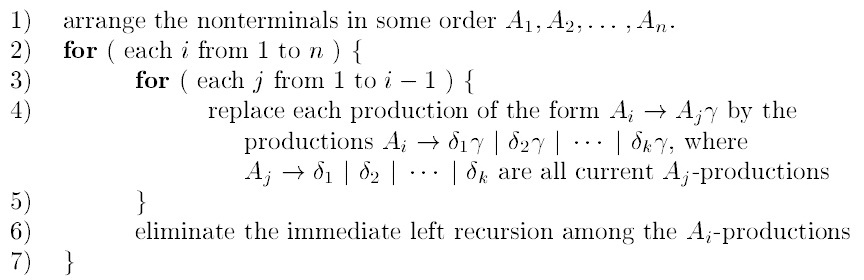
\includegraphics[scale=0.7]{algorithm_left_recursion}
\end{center}
\section{Left factoring}
Many times:
\begin{itemize}
	\item Two alternative production rules have the same prefix
	\item The choice between them is not clear
\end{itemize}
Example: $A\rightarrow \alpha\beta_1|\alpha\beta_2$
\begin{itemize}
	\item Suppose the input begins with a string derived from $\alpha$
	\item Which transition to choose?
	\item We need to read more symbols from the input - this grammar is not an LL(1) grammar
\end{itemize}
We can turn this example into an LL(1) grammar in the following way
$$A\rightarrow \alpha A'$$
$$A' \rightarrow \beta_1|\beta_2$$
\subsection{Algorithm for left factoring}
For each non-terminal A
\begin{itemize}
	\item Find the longest prefix $\alpha$ common to two or more of its alternative productions
	$$A\rightarrow \alpha\beta_1|\alpha\beta_2|...|\alpha\beta_n|\gamma$$
	\item Replace these productions by the following
	$$A\rightarrow \alpha A' | \gamma$$
	$$A'\rightarrow \beta_1|\beta_2|...|\beta_n$$
\end{itemize}
Repeat until no two alternative productions have a common prefix
\section{LL(k) grammars}
When we consider a non-terminal:
\begin{itemize}
	\item How do we know which production rule to use?
	\item The predictive parser looks ahead to the rest of the input and its decision is forced
\end{itemize}
LL(k) grammar:
\begin{itemize}
	\item L: left-to-right scan of the input tokens
	\item L: leftmost derivation of the input string
	\item k: look k tokens ahead in the input string
\end{itemize}
We must first:
\begin{itemize}
	\item Eliminate ambiguities
	\item Eliminate left recursions
	\item Perform left factoring
\end{itemize}
\subsection{LL(1) grammars}
Interesting case:
\begin{itemize}
	\item LL(1) grammars - read only one token ahead in the input
	\item More efficient parsing than other LL(k) grammars
\end{itemize}
How can we uniquely determine the next production in an LL(1) grammar?\\
\\
We do these with the help of two functions (sets)
\begin{itemize}
	\item FIRST($\alpha$), where $\alpha$ is any string of grammar symbols
	\item FOLLOW(A), where A is any non-terminal
\end{itemize}
And a predictive parsing table that associates terminals (of the grammar) with non-terminals (of the input)
\subsubsection{FIRST}
The set FIRST($\alpha$), for a string $\alpha$, contains:
\begin{itemize}
	\item Every first terminal of a string derived from $\alpha$
	\item i.e. if $\alpha\xRightarrow{*} c\gamma$, then $c\in FIRST(\alpha)$
	\item also, if $\alpha\xRightarrow{*} \epsilon$, then $\epsilon\in FIRST(\alpha)$
\end{itemize}
Example usage:
\begin{itemize}
	\item Consider the two productions $A\rightarrow \gamma_1$ and $A\rightarrow \gamma_2$
	\item Suppose that FIRST($\gamma_1$) and FIRST($\gamma_2$) are disjoint
	\item let the next input symbol be a
	\item if a belongs to FIRST($\gamma_1$), then choose $A\rightarrow \gamma_1$
	\item if a belongs to FIRST($\gamma_2$), then choose $A\rightarrow \gamma_2$
	\item Otherwise report error
\end{itemize}
\subsubsection{Follow}
The set FOLLOW(A), for a non-terminal contains:
\begin{itemize}
	\item Every terminal a that can appear immediately to the right of A in some string derived from S
	\item i.e. there exists a derivation $S\xRightarrow{*}\alpha Aa\beta$ where $\alpha$ and $\beta$ are two strings
\end{itemize}
In addition if A can be the rightmost symbol in some string derived from S, then \$ is in FOLLOW(A) (where \$ is the end of file symbol)
\section{LL(1) Grammars}
\begin{definition}[LL(1) Grammar]
A Grammar G is an LL(1) grammar iff for every two productions $A\rightarrow \alpha | \beta$:
\begin{enumerate}
	\item There is no terminal a such that both $\alpha$ and $\beta$ derive a string starting with a
	\item At most one of $\alpha$ and $\beta$ can derive the empty string $\epsilon$
	\item If $\beta \xRightarrow{*}\epsilon$ then $\alpha$ does not derive any string beginning with a terminal in FOLLOW(A) and vice versa
\end{enumerate}
\end{definition}
Therefore an efficient algorithm to determine whether a grammar G is LL(1) grammar by computing all needed sets FIRST() and FOLLOW()\\
\\
A language L is called an LL(1) language is L can be generated by an LL(1) grammar\\
\\
If any language L is given by a non-LL(1) grammar L may still be an LL(1) language by a different grammar
\section{Non-recursive predictive parsing}
We saw predictive parsing via recursive calls of procedures\\
\\
We can "mimic" leftmost derivation:
\begin{itemize}
	\item Explicitly maintain a stack
	\item "table driven predictive parsing"
\end{itemize}
If w is the input that has been matched so far, then the stack holds a sequence $\alpha$ of grammar symbols (terminals and non-terminals), such that
$$S\xRightarrow{*}w\alpha$$
where S is the start symbol of the grammar\\
\\
Given a parsing table M and input w:
\begin{itemize}
	\item Initialise a stack containing S (with bottom symbol \$)
	\item Repeat until the stack contains only \$:
	\begin{itemize}
		\item Let the next input character be c
		\item If the top of the stack is a terminal t, then:
		\begin{itemize}
			\item If c and t don't match, report an error
			\item Otherwise match c and t  - consume c from input and pop t from stack
		\end{itemize}
		\item If the top of the stack is a non-terminal A, then:
		\begin{itemize}
			\item If $M[A,c]$ is undefined, report an error
			\item Otherwise replace the top of the stack with $M[A,c]$
		\end{itemize}
	\end{itemize}
\end{itemize}
\end{document}
